\documentclass[aspectratio=169,11pt]{beamer}
\usepackage[T1]{fontenc}
\usepackage{lmodern,amsmath,amssymb,mathtools,bm,booktabs,array,graphicx,tikz}
\usetikzlibrary{arrows.meta,positioning,calc,decorations.pathreplacing,patterns}
\definecolor{ink}{HTML}{17344D}\definecolor{accent}{HTML}{087E8B}\definecolor{pale}{HTML}{EDF5F5}\definecolor{gold}{HTML}{AD6B19}
\providecommand{\dd}{\,\mathrm{d}}\providecommand{\R}{\mathbb{R}}
\providecommand{\E}{\mathbb{E}}\providecommand{\Var}{\operatorname{Var}}
\providecommand{\Cov}{\operatorname{Cov}}\providecommand{\diag}{\operatorname{diag}}
\providecommand{\norm}[1]{\left\lVert#1\right\rVert}
\providecommand{\abs}[1]{\left|#1\right|}
\usefonttheme{professionalfonts}
\setbeamercolor{normal text}{fg=black,bg=white}
\setbeamercolor{frametitle}{fg=ink,bg=white}
\setbeamercolor{title}{fg=ink}\setbeamercolor{structure}{fg=accent}
\setbeamercolor{block title}{fg=ink,bg=pale}\setbeamercolor{block body}{fg=black,bg=pale!40}
\setbeamercolor{alerted text}{fg=accent}
\setbeamerfont{frametitle}{size=\Large,series=\bfseries}
\setbeamerfont{title}{size=\LARGE,series=\bfseries}
\setbeamertemplate{navigation symbols}{}
\setbeamersize{text margin left=.7cm,text margin right=.7cm}
\setbeamertemplate{frametitle}{\vspace{.18cm}\insertframetitle\par\vspace{.1cm}{\color{accent}\hrule height .6pt}\vspace{.12cm}}
\newcommand{\notestarget}{notes.pdf}\newcommand{\noteslabel}{Notes}
\setbeamertemplate{footline}{\hspace{.7cm}\color{ink}\scriptsize Computational Cardiology\quad\href{\notestarget}{\noteslabel}\hfill\insertframenumber\,/\,\inserttotalframenumber\hspace{.7cm}\vspace{.18cm}}
\setbeamercovered{invisible}
\hypersetup{pdfauthor={Zan Ahmad},pdftitle={Image coordinates, pixel-cell meshes and geometric sensitivity},pdfpagemode=UseNone}
\begin{document}
\begin{frame}[plain]\vfill
{\small\color{accent} Computational Cardiology \quad Lecture 11}\par\medskip
{\raggedright\hyphenpenalty=10000\exhyphenpenalty=10000\LARGE\bfseries\color{ink} Image coordinates, pixel-cell meshes and geometric sensitivity}\par\bigskip
Zan Ahmad\par\smallskip
{\small Fall 2024}\par\vfill\end{frame}
\renewcommand{\notestarget}{notes.pdf\#note-intensity-arrays-and-spatial-metadata}
\begin{frame}[t,fragile,label=slide-an-intensity-array-and-a-geometric-image]{An intensity array and a geometric image}
\[I_{r,c}\in[0,1],\qquad x_{r,c}\in\mathbb R^2.\]\pause{} Intensities do not have length units. Spatial metadata determines physical positions.
\end{frame}
\renewcommand{\notestarget}{notes.pdf\#note-intensity-arrays-and-spatial-metadata}
\begin{frame}[t,fragile,label=slide-thresholding-defines-a-set]{Thresholding defines a set}
\[M_t=\{(r,c):I_{r,c}\ge t\}.\]\pause{} A binary mask defines selected indices before any area is measured.
\end{frame}
\renewcommand{\notestarget}{notes.pdf\#note-the-affine-index-to-physical-map}
\begin{frame}[t,fragile,label=slide-the-physical-coordinate-map]{The physical coordinate map}
\[x=o+D\operatorname{diag}(s_x,s_y)\begin{pmatrix}c\\r\end{pmatrix}.\]\pause{} Array indexing is row--column; the geometric vector is column--row.
\end{frame}
\renewcommand{\notestarget}{notes.pdf\#note-the-affine-index-to-physical-map}
\begin{frame}[t,fragile,label=slide-matrix-order-matters]{Matrix order matters}
\[D\operatorname{diag}(s_x,s_y)\ne\operatorname{diag}(s_x,s_y)D\]\pause{} for unequal spacings and a general rotation.
\end{frame}
\renewcommand{\notestarget}{notes.pdf\#note-the-affine-index-to-physical-map}
\begin{frame}[t,fragile,label=slide-pixel-centers-and-corners]{Pixel centers and corners}
The origin locates the center of pixel zero.\pause{} Corners use $(c\pm\tfrac12,r\pm\tfrac12)$ before the physical transformation.
\end{frame}
\renewcommand{\notestarget}{notes.pdf\#note-the-affine-index-to-physical-map}
\begin{frame}[t,fragile,label=slide-area-scaling]{Area scaling}
\[\det(D\operatorname{diag}(s_x,s_y))=s_xs_y\]\pause{} when $D$ is a proper rotation. Translation does not change area.
\end{frame}
\renewcommand{\notestarget}{notes.pdf\#note-oriented-triangles-and-mask-area}
\begin{frame}[label=slide-triangulating-the-selected-cells-panel-1]{Image +\allowbreak{} threshold mask}
\centering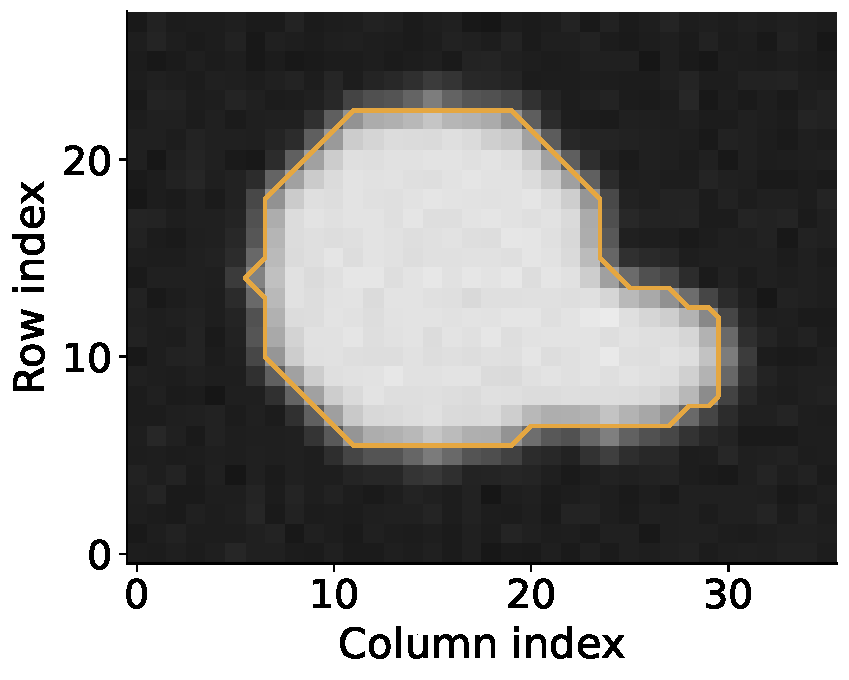
\includegraphics[width=.98\linewidth,height=.69\textheight,keepaspectratio]{presentation-figures/image-mesh-panel-1.pdf}\end{frame}
\renewcommand{\notestarget}{notes.pdf\#note-oriented-triangles-and-mask-area}
\begin{frame}[label=slide-triangulating-the-selected-cells-panel-2]{Two triangles per cell}
\centering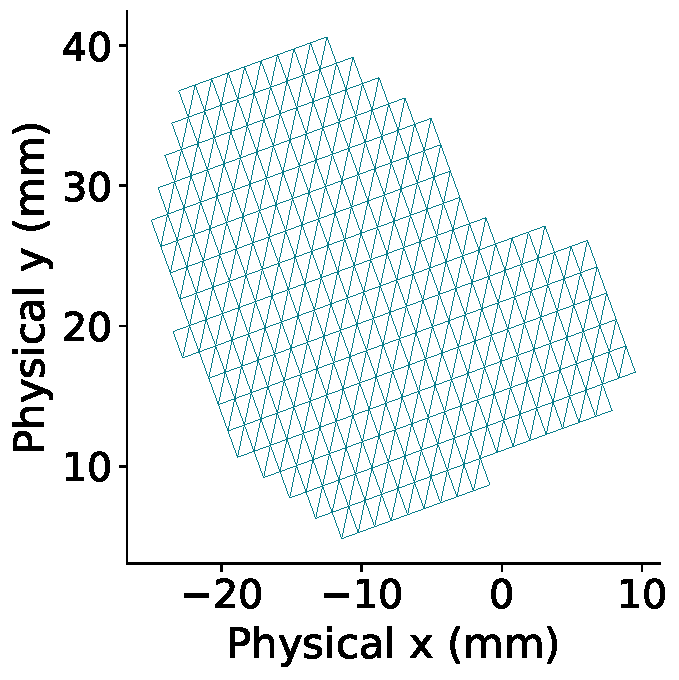
\includegraphics[width=.98\linewidth,height=.69\textheight,keepaspectratio]{presentation-figures/image-mesh-panel-2.pdf}\end{frame}
\renewcommand{\notestarget}{notes.pdf\#note-oriented-triangles-and-mask-area}
\begin{frame}[t,fragile,label=slide-triangulating-the-selected-cells]{Triangulating the selected cells}
Each foreground rectangle becomes two consistently oriented triangles with shared vertex indices.\pause{} This is a mesh of the pixel-cell union.
\end{frame}
\renewcommand{\notestarget}{notes.pdf\#note-oriented-triangles-and-mask-area}
\begin{frame}[t,fragile,label=slide-signed-triangle-area]{Signed triangle area}
\[A_T=\frac12\det\begin{pmatrix}x_2-x_1&x_3-x_1\\y_2-y_1&y_3-y_1\end{pmatrix}.\]\pause{} A sign reversal detects reversed vertex ordering.
\end{frame}
\renewcommand{\notestarget}{notes.pdf\#note-oriented-triangles-and-mask-area}
\begin{frame}[t,fragile,label=slide-mask-area-and-mesh-area]{Mask area and mesh area}
\[A_M=N_f s_xs_y=\sum_TA_T.\]\pause{} The default $295$ selected pixels give $590$ triangles, each of area $1.25$ mm$^2$.
\end{frame}
\renewcommand{\notestarget}{notes.pdf\#note-threshold-sets-and-geometric-summaries}
\begin{frame}[label=slide-threshold-sets-are-nested-panel-1]{Segmentation sensitivity}
\centering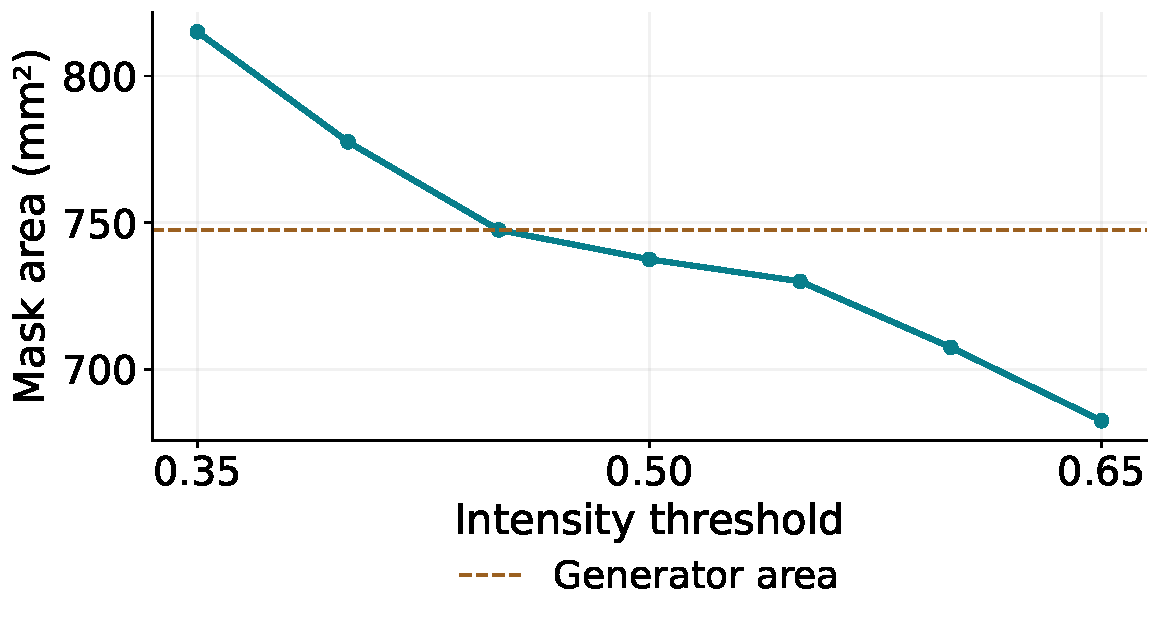
\includegraphics[width=.98\linewidth,height=.69\textheight,keepaspectratio]{presentation-figures/geometry-sensitivity-panel-1.pdf}\end{frame}
\renewcommand{\notestarget}{notes.pdf\#note-threshold-sets-and-geometric-summaries}
\begin{frame}[label=slide-threshold-sets-are-nested-panel-2]{Equivalent-circle summary}
\centering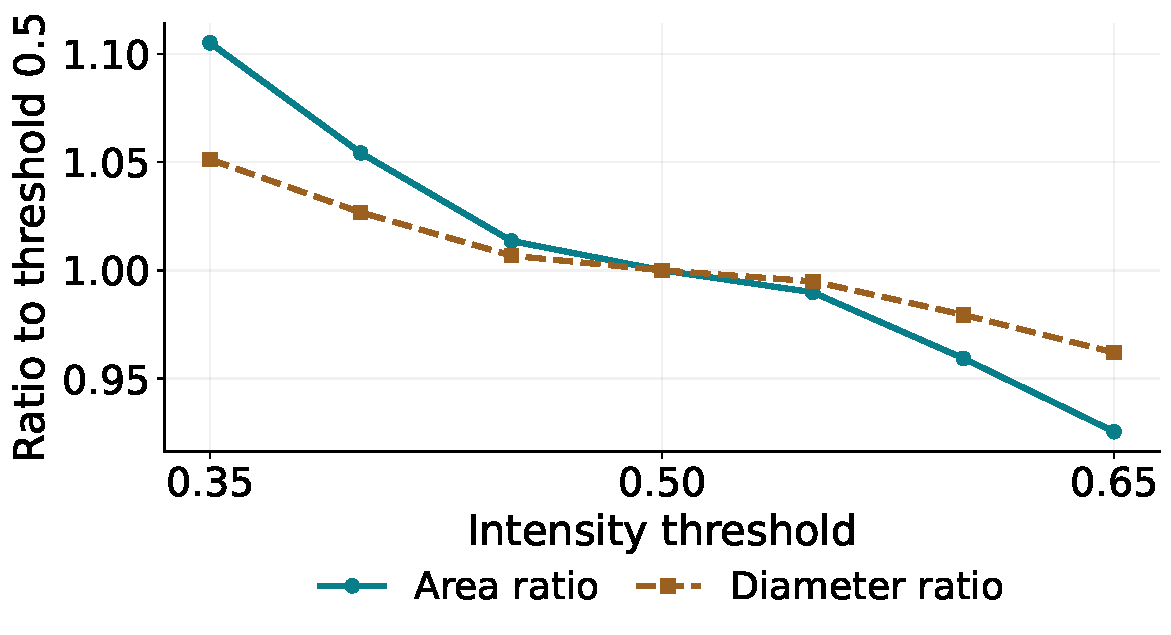
\includegraphics[width=.98\linewidth,height=.69\textheight,keepaspectratio]{presentation-figures/geometry-sensitivity-panel-2.pdf}\end{frame}
\renewcommand{\notestarget}{notes.pdf\#note-threshold-sets-and-geometric-summaries}
\begin{frame}[t,fragile,label=slide-threshold-sets-are-nested]{Threshold sets are nested}
\[t_2>t_1\quad\Longrightarrow\quad M_{t_2}\subseteq M_{t_1}.\]\pause{} Area cannot increase, but component count need not be monotone.
\end{frame}
\renewcommand{\notestarget}{notes.pdf\#note-threshold-sets-and-geometric-summaries}
\begin{frame}[t,fragile,label=slide-equivalent-circle-diameter]{Equivalent-circle diameter}
\[d_{eq}=2\sqrt{A_M/\pi}.\]\pause{} This is an area summary, not an estimate of every anatomical diameter.
\end{frame}
\renewcommand{\notestarget}{notes.pdf\#note-threshold-sets-and-geometric-summaries}
\begin{frame}[t,fragile,label=slide-relative-sensitivity]{Relative sensitivity}
\[\frac{\delta d_{eq}}{d_{eq}}\simeq\frac12\frac{\delta A}{A}.\]\pause{} A threshold range is not a confidence interval without a probability model.
\end{frame}
\renewcommand{\notestarget}{notes.pdf\#note-representation-error-and-physical-interpretation}
\begin{frame}[t,fragile,label=slide-scale-and-location-have-different-signatures]{Scale and location have different signatures}
Doubling both spacings quadruples area.\pause{} Translating the origin changes all positions while preserving every triangle area.
\end{frame}
\renewcommand{\notestarget}{notes.pdf\#note-representation-error-and-physical-interpretation}
\begin{frame}[t,fragile,label=slide-refining-the-mesh-does-not-refine-the-image]{Refining the mesh does not refine the image}
Subdividing triangles inside the same selected cells leaves the represented boundary unchanged.\pause{} Resolving a finer boundary requires additional image information or a new geometric assumption.
\end{frame}
\renewcommand{\notestarget}{notes.pdf\#note-resampling-and-geometric-provenance}
\begin{frame}[t,fragile,label=slide-label-resampling]{Label resampling}
Nearest-neighbor resampling preserves the set of label values.\pause{} It need not preserve thin connections, area or boundary position on a new target grid.
\end{frame}
\end{document}
